%\documentclass[10pt]{beamer}
\documentclass[10pt,aspectratio=169,usenames,dvipsnames]{beamer}

\usetheme[progressbar=frametitle]{metropolis}
\usepackage{appendixnumberbeamer}

\usepackage{booktabs}
\usepackage[scale=2]{ccicons}

\usepackage{pgfplots}
\usepgfplotslibrary{dateplot}

\usepackage{xspace}
\newcommand{\themename}{\textbf{\textsc{metropolis}}\xspace}

\usepackage{graphicx}

\setbeamertemplate{enumerate items}[circle]

\usepackage{pict2e}

\usepackage{media9}

%\usepackage{multimedia} %for the movie
\usepackage{media9} %for the movie

\usepackage{amsmath}

\usepackage{mathtools}
\DeclarePairedDelimiter\abs{\lvert}{\rvert}%
\DeclarePairedDelimiter\norm{\lVert}{\rVert}%
\makeatletter
\let\oldabs\abs
\def\abs{\@ifstar{\oldabs}{\oldabs*}}

\usepackage[makeroom]{cancel}

\usepackage{xcolor}
\usepackage{soul}
\newcommand{\mathcolorbox}[2]{\colorbox{#1}{$\displaystyle #2$}}

\title{MHD shocks and turbulence in the Orszag-Tang vortex}
%ABSTRACT: Compressible magnetohydrodynamic (MHD) turbulence is a common feature of astrophysical systems such as the solar atmosphere and interstellar medium. Such systems are rife with shock waves that can redistribute and dissipate energy, and hence understanding the role of shocks in compressible turbulence is critical for determining the energy balance of these dynamic systems. However, automated detection and classification of shocks in turbulent systems is inherently difficult due to the highly dynamic medium. Here we present a method for detecting and classifying the full range of MHD shocks (slow, fast and intermediate) applied to the Orszag-Tang vortex. In particular, intermediate shocks (which feature a reversal in the magnetic field) appear to form most readily near reconnection sites. We present a potential mechanism that could lead to the formation of intermediate shocks in MHD systems and the role of shocks in redistributing and dissipating energy in compressible MHD turbulence.
\date{}
\author{\textbf{Ben Snow$^1$}, A. Hillier$^1$, G. Murtas$^1$, J. Mason$^1$, G. J. J. Botha$^2$}
\institute{$^1$University of Exeter, $^2$ Northumbria University \\ NAM2023, July 2023.}

\begin{document}

\maketitle

\begin{frame}{Turbulence in astrophysics}
% \begin{itemize}
%     \item Turbulence is a fundamental feature of astrophysical systems
% %    \item Substructure possible.
% \end{itemize}
\begin{columns}
\begin{column}{0.5\textwidth}
%\includegraphics[width=0.95\linewidth]{spot.jpg} Sunspot simulation, Rempel+2009 REPLACE
\includegraphics[width=0.95\linewidth]{Rempel_divv.png} Photospheric granulation (horizontal flow divergence), Rempel+2018
%\includegraphics[width=1.0\textwidth,clip=true,trim=1.0cm 1.0cm 1.0cm 1.0cm]{obs_shockloc_contour.png}
\end{column}
\begin{column}{0.5\textwidth}
\includegraphics[width=0.95\linewidth]{crab-nebula-mosaic.jpg} Crab Nebula,  (NASA, ESA, J. Hester and A. Loll (Arizona State University))
\end{column}
\end{columns}
\end{frame}

\begin{frame}{Compressible turbulence}
\begin{columns}
\begin{column}{0.4\textwidth}
\begin{enumerate}
\item Early turbulence work assumed solenoidal velocity or constant density/temperature.
\item These conditions not usually suitable for astrophysical systems.
\item Shocks are an example of highly compressible effects.
\item Understanding shocks is fundamental to understanding dissipation and energy transfer in compressible turbulence.
\end{enumerate}
\end{column}
\begin{column}{0.6\textwidth}
%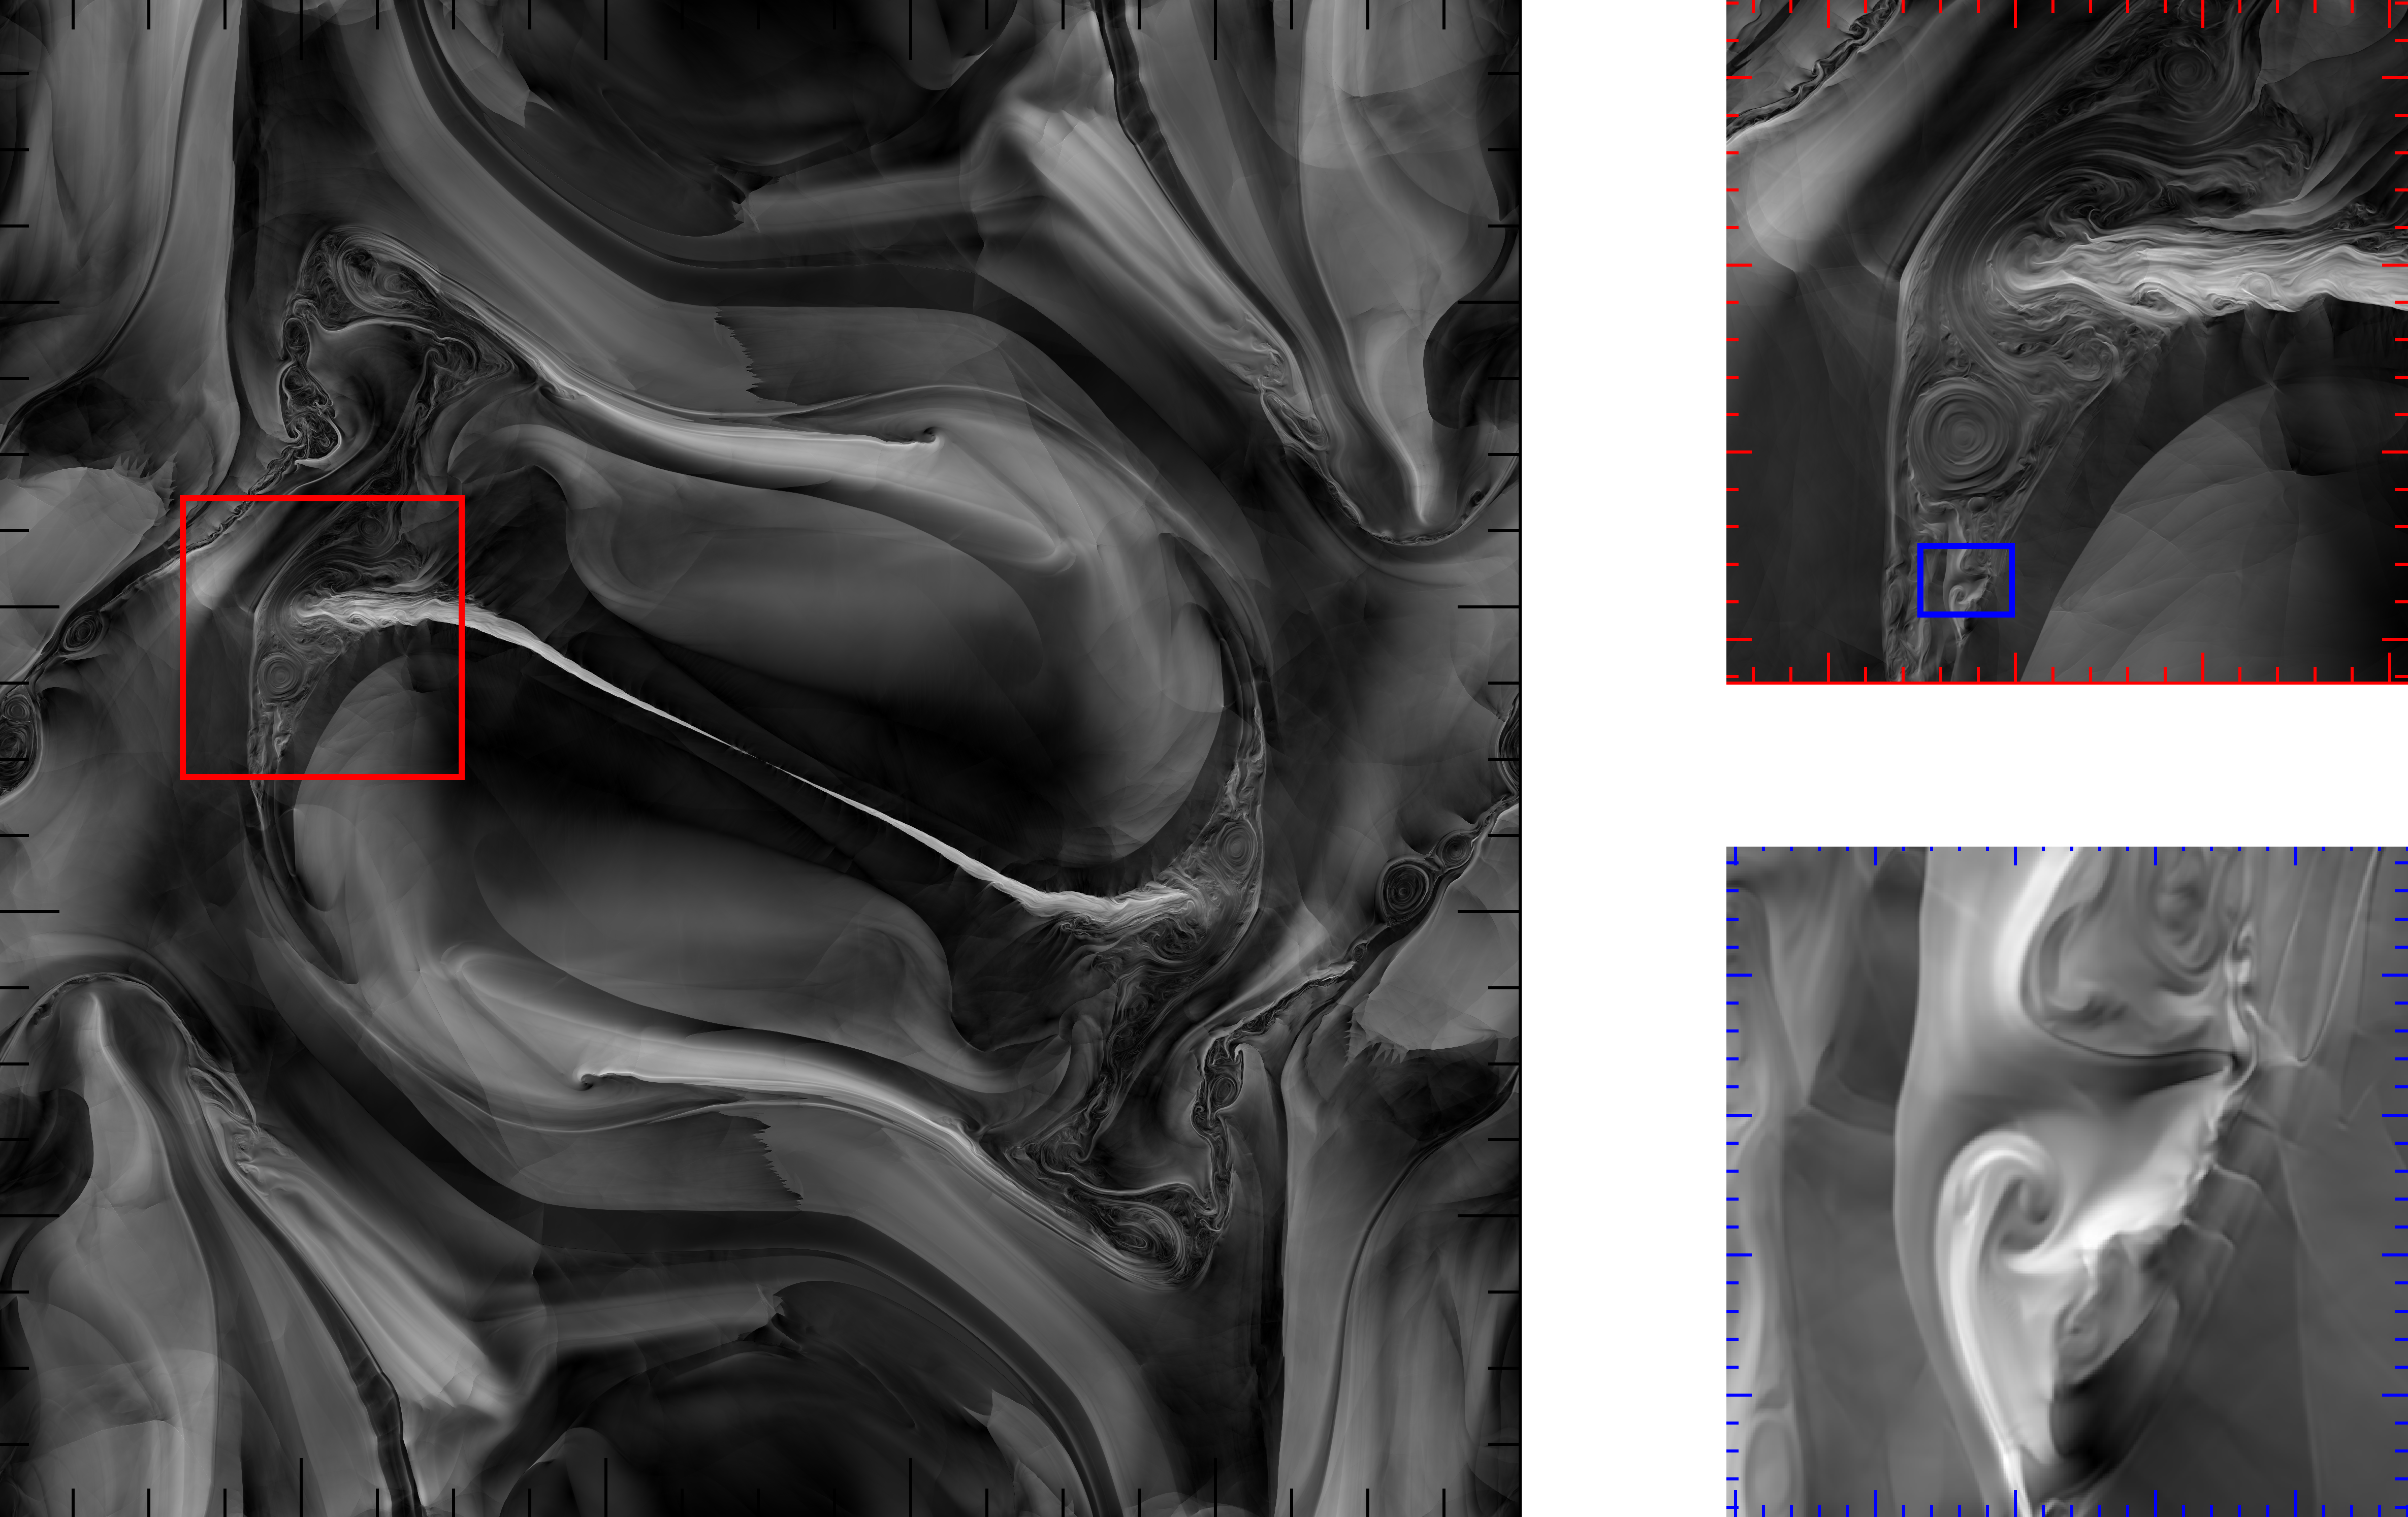
\includegraphics[width=0.95\textwidth]{contextplot_MHD.png}
\includegraphics[width=0.95\textwidth,clip=true,trim=3.8cm 7.4cm 2.5cm 7.5cm]{MHD_1024_ro.pdf}
\end{column}
\end{columns}
\end{frame}

% \begin{frame}{Shocks in MHD}
% %\begin{columns}
% %\begin{column}{0.6\textwidth}
% \begin{enumerate}
% \item MHD has three characteristic wave speeds (slow, Alfv\'en, fast).
% %\item Multiple transitions possible.
% %\item Finite shock width in two-fluid allows substructure to exist.
% %\item Slow-mode shock is a transition from super-slow to sub-slow.
% %\item Important for reconnection, e.g., Petschek-like.
% \item Intermediate shocks feature a reversal in the magnetic field across the interface.
% \end{enumerate}
% %\end{column}
% %\begin{column}{0.5\textwidth}
% %\end{column}
% %\end{columns}
% \begin{columns}
% \begin{column}{0.5\textwidth}
% \begin{itemize}
% \item (1) superfast: $V_f < \abs{v_n}$,
% %\item (1=2) fast: $\abs{v_n} = V_f$,
% \item (2) subfast: $V_A < \abs{v_n} < V_f $,
% %\item (2=3) Alfv\'en: $\abs{v_n} = V_A$,
% \item (3) superslow: $V_s < \abs{v_n} < V_A$,
% %\item (3=4) slow: $V_s = \abs{v_n}$,
% \item (4) subslow: $0< \abs{v_n} < V_s$,
% \item ($\infty$) static: $v_n = 0$.
% \end{itemize}
% \end{column}
% \begin{column}{0.5\textwidth}
% \begin{itemize}
% \item $1 \rightarrow 2 $ fast shocks
% \item $3 \rightarrow 4$ slow shocks
% % \item $1 \rightarrow 2=3$ switch-on
% % \item $2=3 \rightarrow 4$ switch-off
% \item $1\rightarrow 3, 1 \rightarrow 4, 2 \rightarrow 3, 2 \rightarrow 4$ intermediate shocks
% \end{itemize}
% \end{column}
% \end{columns}
% \end{frame}

\begin{frame}{Shock transitions}
\begin{columns}
\begin{column}{0.4\textwidth}
\begin{itemize}
    \item Stable shock solutions can be analytically determined by the upstream plasma-$\beta$, angle of magnetic field $\theta$, and Alfven Mach numbers.
\end{itemize}
\end{column}
\begin{column}{0.6\textwidth}
\includegraphics[width=0.95\linewidth,clip=true,trim=1.0cm 8.0cm 2.5cm 8.5cm]{shockjumps_0.125pi.pdf}
\end{column}
\end{columns}
\begin{gather}
    A_\perp ^{\text{u}2} = \frac{ A_\perp ^{\text{d}2} \left( \frac{\gamma-1}{\gamma} \left( \frac{\gamma+1}{\gamma -1} -\tan ^2 \theta \right) \left(A_\perp ^{\text{d}2} -1 \right) ^2 + \tan ^2 \theta  \left( \frac{\gamma-1}{\gamma} A_\perp ^{\text{d}2} -1 \right) \left(A_\perp ^{\text{d}2} -2 \right) \right) - \frac{\beta }{ \cos ^2 \theta } \left( A_\perp ^{\text{d}2} -1 \right) ^2 } { \frac{\gamma -1}{\gamma} \frac{\left( A_\perp ^{\text{d}2}-1 \right) ^2}{ \cos ^2 \theta ^{\text{u}}} - A_ \perp ^{\text{d}2} \tan ^2 \theta ^{\text{u}} \left( \frac{\gamma -1}{\gamma} A_\perp ^{\text{d}2} -1 \right) } \label{eqn:hau}
\end{gather}
\begin{flushright}
{\small Hau+1989}
\end{flushright}
\end{frame}

\begin{frame}{Shock detection}
\begin{columns}
\begin{column}{0.4\textwidth}
\begin{enumerate}
\item What types of shocks are being created?
\item Where are the shocks?
\item What do the shocks tell us about the system?
\item Automated detection from simulation.
\end{enumerate}
\end{column}
\begin{column}{0.6\textwidth}
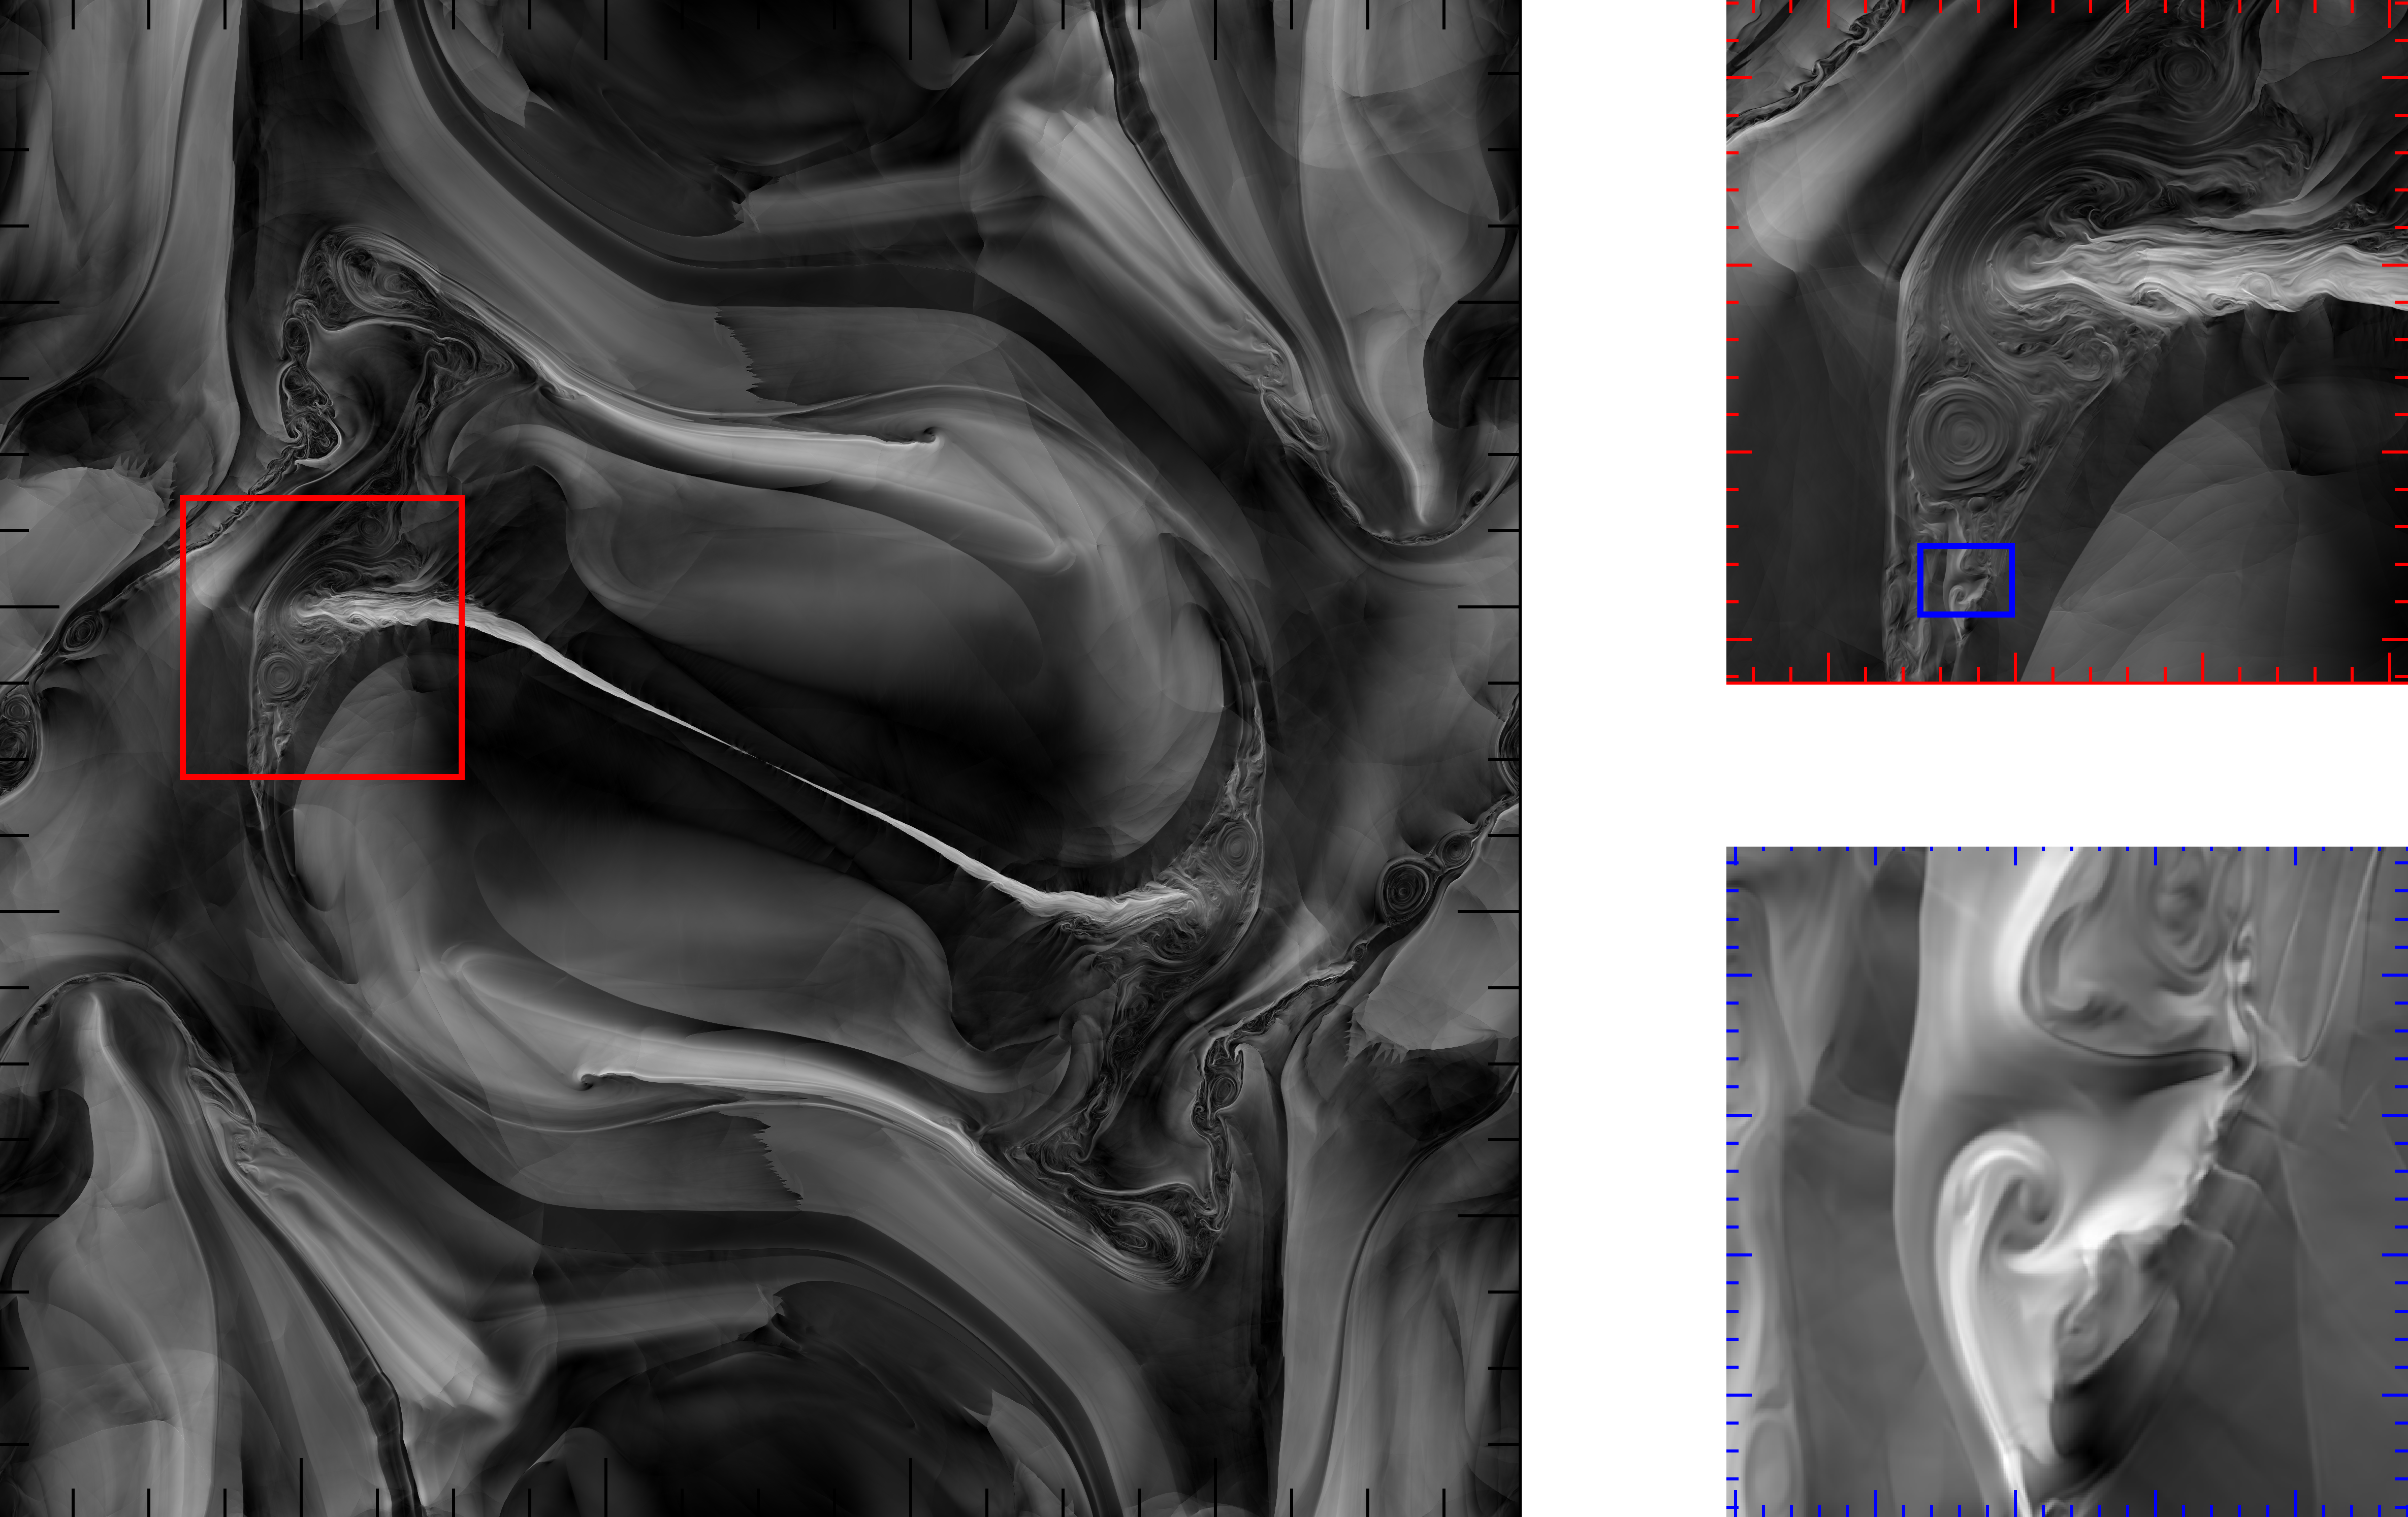
\includegraphics[width=0.95\textwidth]{contextplot_MHD.png}
\end{column}
\end{columns}
\end{frame}

\begin{frame}{Detection method}
\begin{enumerate}
    \item Identify shock candidates based on the divergence of the velocity field 
    %($\nabla \cdot \textbf{v} < 0$ is a necessary condition for a shock). 
    \item Calculate the parallel and perpendicular unit vectors based on the maximum density gradient.
    %The list of possible shocks is then filtered by checking the density gradient along a line perpendicular to the shock front. If the possible shock is not a local maxima of minima of the perpendicular density gradient, then it is not the centre of the feature and is discarded. This prevents the numerical (and physical) finite width of the shock resulting in multiple detections.
    \item Estimate the shock frame from the steady-state conservation of mass equation. 
    %In the deHoffman-Teller shock frame, the conservation of mass equation becomes $\left[ \rho v_\perp \right]^u _d =0$. To transfer the simulation laboratory frame to the shock frame, we need the shock velocity $v_s$. However, this is difficult to determine from a static 2D snapshot. By rewriting the mass conservation including this constant shock velocity as $\left[ \rho (v_\perp+v_s) \right]^u _d =0$, where $v_\perp$ is directly from the simulation, we can estimate the shock velocity by rearranging as $v_s=\frac{\rho ^d v_{\perp}^d-\rho ^u v_{\perp}^u}{\rho^u-\rho^d}$. There are a number of assumptions that go into this formulation, namely that the shock is steady-state. In a highly dynamic simulation, this may prevent transient shocks being detected as readily and could lead to erroneous shock detection. 
    \item Calculate the upstream and downstream slow, Alfv\'en and fast Mach numbers. 
    \item Compare the upstream and downstream states to calculate the shock transition. 
    %The upstream and downstream directions are determined by the density requirement that, for a shock, $\rho^d>\rho^u$. This ensures a compressibility of $r>1$, required for a steady-state shock. An extra check is performed here to ensure that the detected intermediate shocks feature a reversal in magnetic field across the interface. 
\end{enumerate}

There are a number of assumptions that go into this identification technique, with the strongest being that the shocks are steady-state. In a turbulent system there are likely to be many shocks that have not yet reached their steady-condition, or are interacting with other features. As such, our identification procedure is likely an underestimate of the number of shocks in the system. Our strict classification helps prevent false detections.
\end{frame}

\begin{frame}{Application - Orszag-Tang Vortex}
\begin{columns}
\begin{column}{0.4\textwidth}
\begin{gather}
    v_{x}=-v_0 \sin (2 \pi y) \\
    v_{y}= v_0 \sin (2 \pi x) \\
    B_{x}=-B_0 \sin (2 \pi y) \\
    B_{y}= B_0 \sin (4 \pi y) \\
    \rho = 25/(36 \pi) \\
    P=5/(12 \pi) \\
    v_0=1 \\
    B_0=1/\sqrt{4 \pi}
\end{gather}
\end{column}
\begin{column}{0.6\textwidth}
\includegraphics[width=0.95\textwidth,clip=true,trim=3.8cm 7.4cm 2.5cm 7.5cm]{MHD_1024_ro.pdf}
\begin{enumerate}
    \item Decaying compressible turbulence (with lots of shocks).
\end{enumerate}
\end{column}
\end{columns}
\end{frame}

% \begin{frame}{Application - Orszag-Tang Vortex}
% \includegraphics[width=0.65\textwidth,clip=true,trim=3.8cm 7.4cm 2.5cm 7.5cm]{MHD_1024_ro.pdf} 
% \end{frame}

% \begin{frame}{Application - Orszag-Tang Vortex}
% \includegraphics[width=0.65\textwidth,clip=true,trim=3.8cm 7.4cm 2.5cm 7.5cm]{MHD_1024_conv.pdf}
% \end{frame}

% \begin{frame}{Application - Orszag-Tang Vortex}
% \includegraphics[width=0.65\linewidth,clip=true,trim=3.8cm 8.4cm 2.5cm 8.5cm]{shockid_PIP_MHD_t100.pdf}
% \end{frame}

\begin{frame}{Movie}
% \movie[width = 0.9\linewidth,height = 0.9\linewidth,  showcontrols]{Movie}{shockid_PIP_movie_MHD.mp4}
%\includemedia[width = 0.9\linewidth]{Movie}{shockid_PIP_movie_MHD.mp4}
\end{frame}

\begin{frame}{Time series of shocks}
    \includegraphics[width=0.32\linewidth,clip=true,trim=3.8cm 8.4cm 2.5cm 8.5cm]{shockid_PIP_MHD_t30.pdf}
    \includegraphics[width=0.32\linewidth,clip=true,trim=3.8cm 8.4cm 2.5cm 8.5cm]{shockid_PIP_MHD_t50.pdf} 
    \includegraphics[width=0.32\linewidth,clip=true,trim=3.8cm 8.4cm 2.5cm 8.5cm]{shockid_PIP_MHD_t60.pdf} \\
    \includegraphics[width=0.32\linewidth,clip=true,trim=3.8cm 8.4cm 2.5cm 8.5cm]{shockid_PIP_MHD_t80.pdf} 
    \includegraphics[width=0.32\linewidth,clip=true,trim=3.8cm 8.4cm 2.5cm 8.5cm]{shockid_PIP_MHD_t100.pdf}
    \includegraphics[width=0.32\linewidth,clip=true,trim=2.8cm 8.3cm 2.5cm 8.5cm]{shockcounts_MHD.pdf} %\\ MHD SHOCK-SHOCK INTERACTION?
\end{frame}

\begin{frame}{Corrugation instability}
\begin{columns}
\begin{column}{0.5\textwidth}
\includegraphics[width=0.9\textwidth]{park2019shocks.png}
\begin{enumerate}
    \item Park+2019 state that the corrugation instability prevents slow-shocks being detected in their turbulent simulations.
    \item Corrugation instability increases length of the shock front and results in more pixel detection.
\end{enumerate}
\end{column}
\begin{column}{0.5\textwidth}
\includegraphics[width=0.95\linewidth,clip=true,trim=1.0cm 10.0cm 2.5cm 10.0cm]{shockstabtest5.pdf} \\
\includegraphics[width=0.95\linewidth,clip=true,trim=1.0cm 10.0cm 2.5cm 10.0cm]{shockstabtest5b.pdf} \\ {\small Snow+2021 (submitted)}
\end{column}
\end{columns}
\end{frame}

\begin{frame}{Intermediate shocks}
\includegraphics[width=0.95\textwidth,clip=true,trim=1.0cm 9.5cm 2.0cm 10.0cm]{recregion2_multi2_plot.pdf}
%\includegraphics[width=0.95\textwidth,clip=true,trim=0.5cm 2.4cm 2.0cm 3.0cm]{recregion2_multi2_plot.png}
% \begin{columns}
% \begin{column}{0.4\textwidth}
\begin{enumerate}
\item Intermediate shocks form at high-current regions.
\end{enumerate}
% \end{column}
% \begin{column}{0.6\textwidth}
% \includegraphics[width=0.95\textwidth,clip=true,trim=0.0cm 2.4cm 0.0cm 2.5cm]{recregion2_multi.pdf}
% \end{column}
% \end{columns}
\end{frame}

\begin{frame}{Plasmoid formation}
\begin{columns}
\begin{column}{0.4\textwidth}
\includegraphics[width=0.95\textwidth]{zenitani_ex.png} \\ 
\includegraphics[width=0.95\textwidth]{zenitani_schem.png} \\ {\small figure from Zenitani+2014}
\end{column}
\begin{column}{0.6\textwidth}
%\includegraphics[width=0.95\textwidth,clip=true,trim=3.0cm 8.5cm 4.0cm 8.0cm]{plasmoid_ex.pdf}
\scalebox{-1}[1]{\includegraphics[width=0.95\textwidth,clip=true,trim=3.0cm 8.5cm 4.0cm 8.0cm]{hrplasmoid_t100.pdf}}
%\includegraphics[width=0.95\textwidth,clip=true,trim=3.0cm 8.5cm 4.0cm 8.0cm]{hrplasmoid3.pdf}
\end{column}
\end{columns}
\end{frame}

\begin{frame}{Potential formation mechanism}
\begin{columns}
\begin{column}{0.5\textwidth}
\includegraphics[width=0.95\textwidth]{Wu_petscheck_drawing.jpg} \\ {\small figure from Wu+1996}
\begin{enumerate}
\item Petschek reconnection features switch-off slow mode shocks (Petschek 1964)
\item Slight perturbation to inflow conditions could produce intermediate shock.
\end{enumerate}
\end{column}
\begin{column}{0.5\textwidth}
\includegraphics[width=0.95\linewidth,clip=true,trim=1.0cm 8.0cm 2.5cm 8.5cm]{shockjumps_0.125pi.pdf} \\
\includegraphics[width=0.95\textwidth]{shockschem.png}
\end{column}
\end{columns}
\end{frame}

\begin{frame}{Conclusions}
\begin{itemize}
    \item Developed method for automated detection and classification of shocks..
    \item Analysed shock formation in Orszag-Tang vortex.
    \item System dominated by fast and slow shocks.
    \item Detected intermediate shocks near reconnection regions.
    \item Intermediate shocks have enhanced current across the interface - more efficient energy dissipation? particle acceleration?
    \item Potential mechanism related to the turbulent inflow to reconnection region.
    \item Is this a common feature?
\end{itemize}
\end{frame}

\begin{frame}{Plasmoid formation}
%\includegraphics[width=0.4\textwidth]{zenitani_schem.png}
\includegraphics[width=0.95\textwidth,clip=true,trim=3.0cm 11cm 4.0cm 11cm]{hrplasmoid3.pdf}
\end{frame}

\end{document}
